% !TeX encoding = UTF-8
% !TeX root = master.tex
% !TeX spellcheck = en_US

\documentclass[aspectratio=43,xcolor=x11names,compress]{beamer}

%---------------------------------------------------------------------------------------------------
% Beamer configuration
%---------------------------------------------------------------------------------------------------

\usepackage{etoolbox}

\newtoggle{safetymargin}
\togglefalse{safetymargin}

\iftoggle{safetymargin}{
	\geometry{paperwidth=128mm,paperheight=96mm}
	\usepackage[width=138mm,height=106mm,frame,noinfo]{crop}
	\voffset\stockheight
	\advance\voffset-\paperheight
	\voffset.5\voffset
	\hoffset\stockwidth
	\advance\hoffset-\paperwidth
	\hoffset.5\hoffset
}


\setbeamertemplate{footline}[page number]{}
\setbeamerfont{footline}{size=\fontsize{8}{10}\selectfont}
\setbeamertemplate{navigation symbols}{}
\setbeamertemplate{caption}[numbered]

\useoutertheme[subsection=false,shadow]{miniframes}
\useinnertheme{default}
\usefonttheme{serif}

\setbeamerfont{title like}{shape=\scshape}
\setbeamerfont{frametitle}{shape=\scshape}

\setbeamercolor*{lower separation line head}{bg=DeepSkyBlue4}
\setbeamercolor*{normal text}{fg=black,bg=white}
\setbeamercolor*{alerted text}{fg=red}
\setbeamercolor*{example text}{fg=black}
\setbeamercolor*{structure}{fg=black}

\setbeamercolor*{palette tertiary}{fg=black,bg=black!10}
\setbeamercolor*{palette quaternary}{fg=black,bg=black!10}

\renewcommand{\(}{\begin{columns}}
\renewcommand{\)}{\end{columns}}
\newcommand{\<}[1]{\begin{column}{#1}}
	\renewcommand{\>}{\end{column}}

%\setbeamersize{text margin left=10mm}
%\setbeamersize{sidebar width left=5mm}


%---------------------------------------------------------------------------------------------------
% Packages
%---------------------------------------------------------------------------------------------------

\usepackage{mathpazo}
\usepackage[utf8]{inputenc}
\usepackage[T1]{fontenc}
\usepackage[english]{babel}
\selectlanguage{english}
\usepackage{graphicx}
\usepackage{grffile}
\graphicspath{{figures/}}
\usepackage{float}
\usepackage{booktabs}
\usepackage{tabu}
\usepackage{rotating}
\usepackage{array}
\usepackage{multirow}
\usepackage{url}
\usepackage{hyperref}
\usepackage[capitalise,noabbrev,nameinlink]{cleveref}
\usepackage[nonumberlist,acronym,nomain,nowarn]{glossaries}
\usepackage[gen]{eurosym}
\usepackage[center]{caption}
\captionsetup{font=footnotesize,labelfont=footnotesize}
\captionsetup[figure]{name=Fig.,indention=0pt}
\glsdisablehyper
\makeglossaries

\makeatletter
\g@addto@macro{\UrlBreaks}{\UrlOrds}
\makeatother

%\overfullrule=3mm

%\newacronym{latex-label}{acronym}{acronym description}



%---------------------------------------------------------------------------------------------------
% Top matter
%---------------------------------------------------------------------------------------------------

\title{Human-robot cooperative assembly with semantic learning by demonstration}
\subtitle{ProDEI - Research Planning}
\author{Carlos M. Costa\texorpdfstring{\\{\ttfamily carlos.costa@fe.up.pt}}{}}
\institute{
	\footnotesize {
		\emph{Supervisor: } Germano Manuel Correia dos Santos Veiga (PhD)\\
		\emph{Co-supervisor: } Armando Jorge Miranda de Sousa (PhD)
	}\\
	\vspace{0.7em}
	INESC TEC and Faculty of Engineering, University of Porto, Portugal\\
}
\date{July 26, 2016}


\begin{document}

\begin{frame}
	\titlepage
\end{frame}



%---------------------------------------------------------------------------------------------------
% Outline
%---------------------------------------------------------------------------------------------------

\begin{frame}{Presentation Outline}
	\begingroup
	\scriptsize
	\tableofcontents
	\endgroup
\end{frame}



%---------------------------------------------------------------------------------------------------
% Sections
%---------------------------------------------------------------------------------------------------

\section{\scshape Introduction}\label{sec:introduction}

\subsection{Context}
\begin{frame}{Context}
	\begin{itemize}
		\item Assembly of complex objects by robots requires long programming periods
		\item Most industrial robots are programmed to perform a very specific task in a controlled environment
		\begin{figure}[!ht]
			\centering
			\begin{minipage}{.35\textwidth}
				\centering
				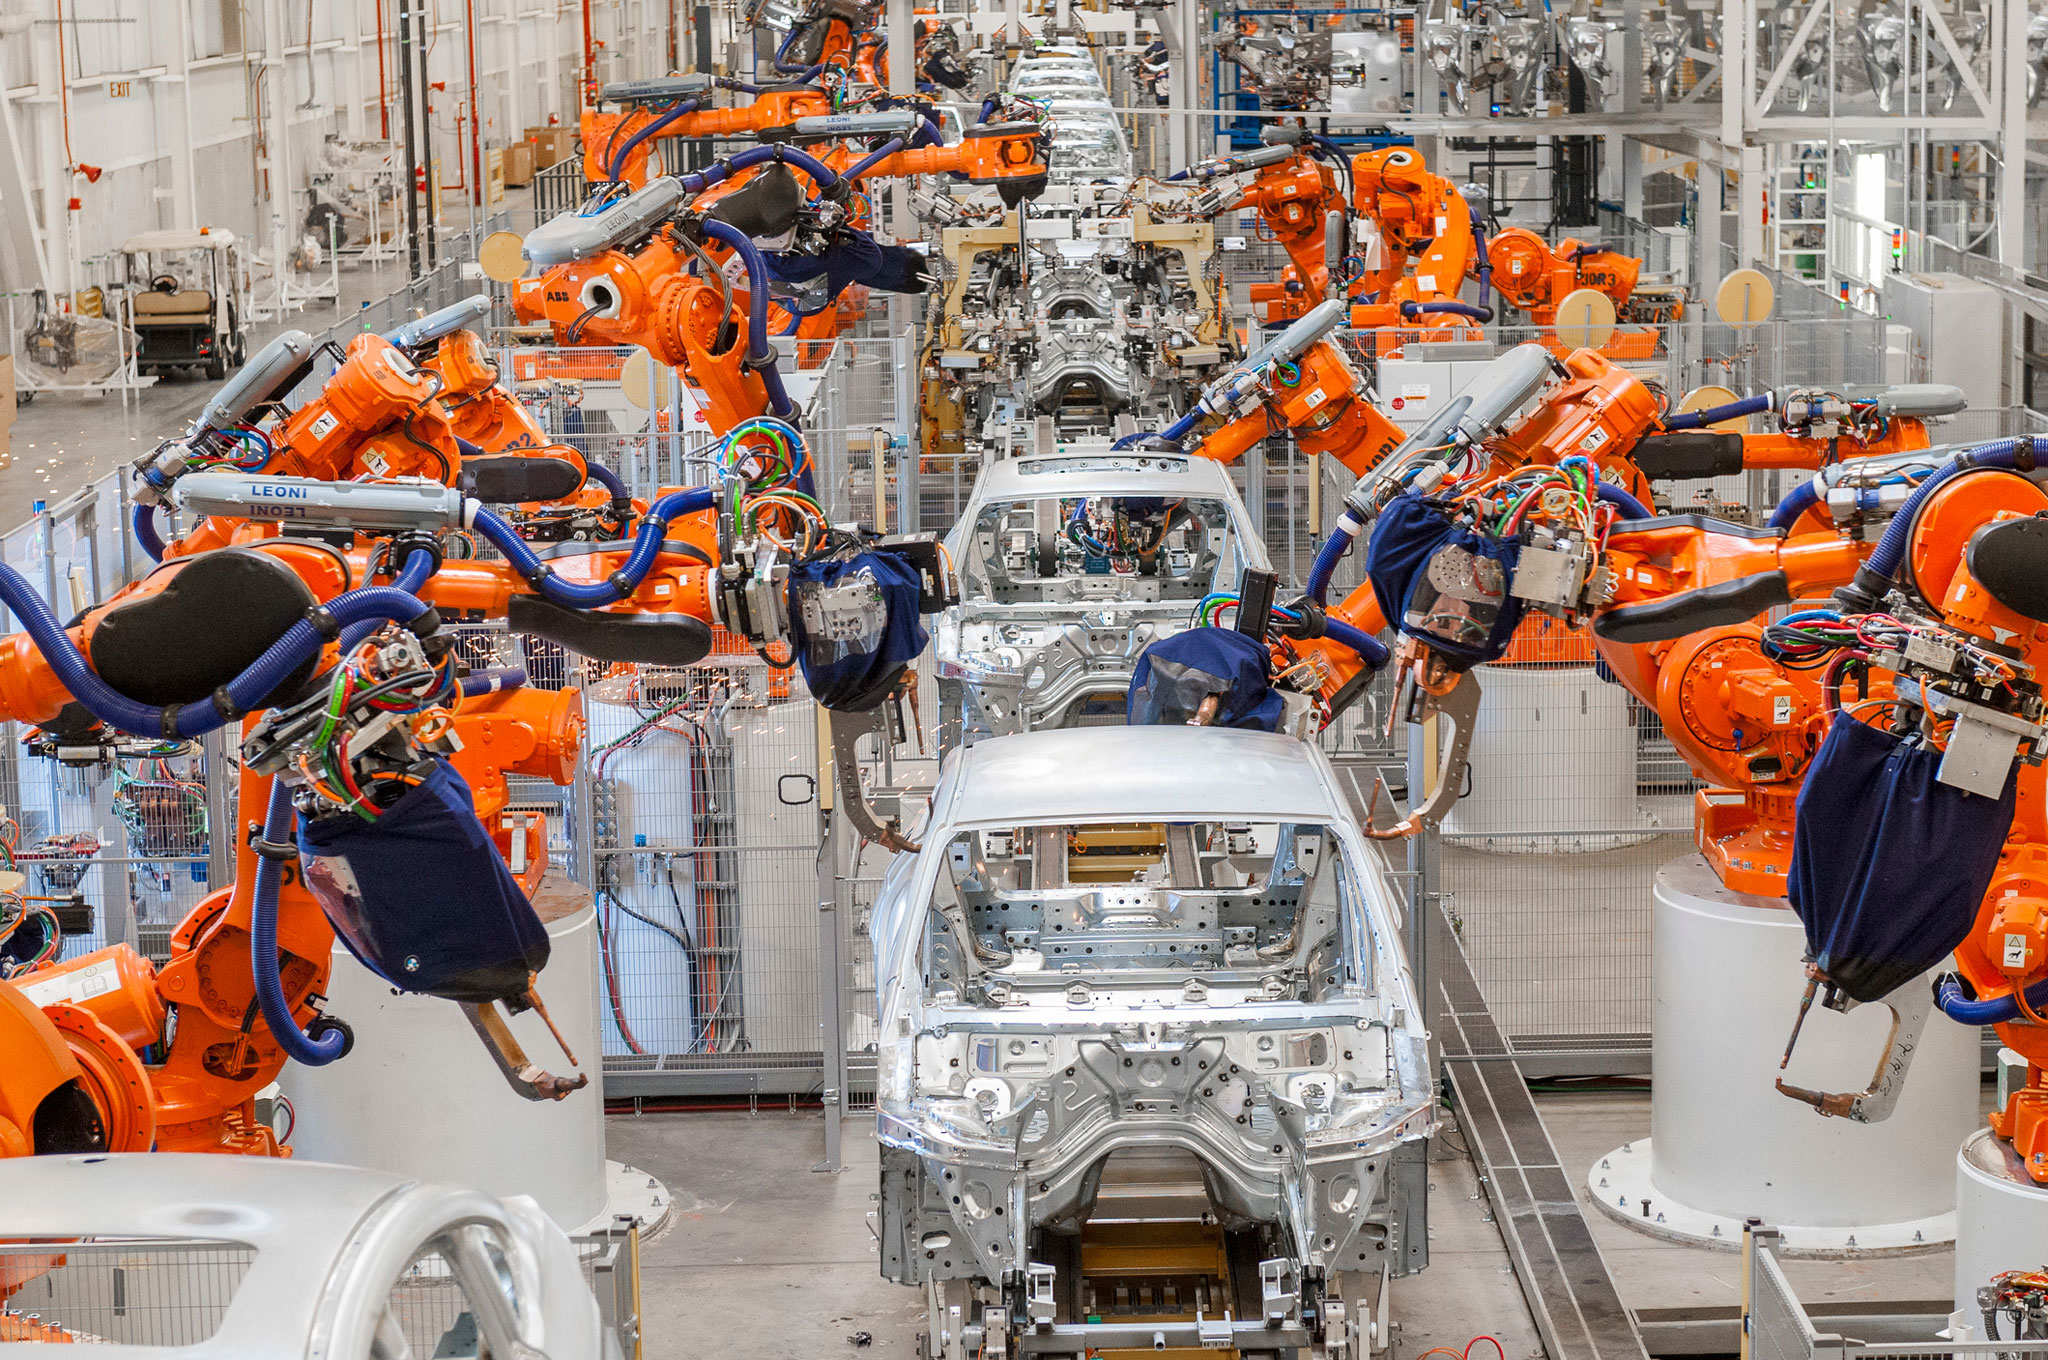
\includegraphics[height=.3\textheight]{bmw-spartanburg-robotic-welding-line}
				\caption{Car assembly line}
			\end{minipage}%
			\begin{minipage}{0.60\textwidth}
				\centering
				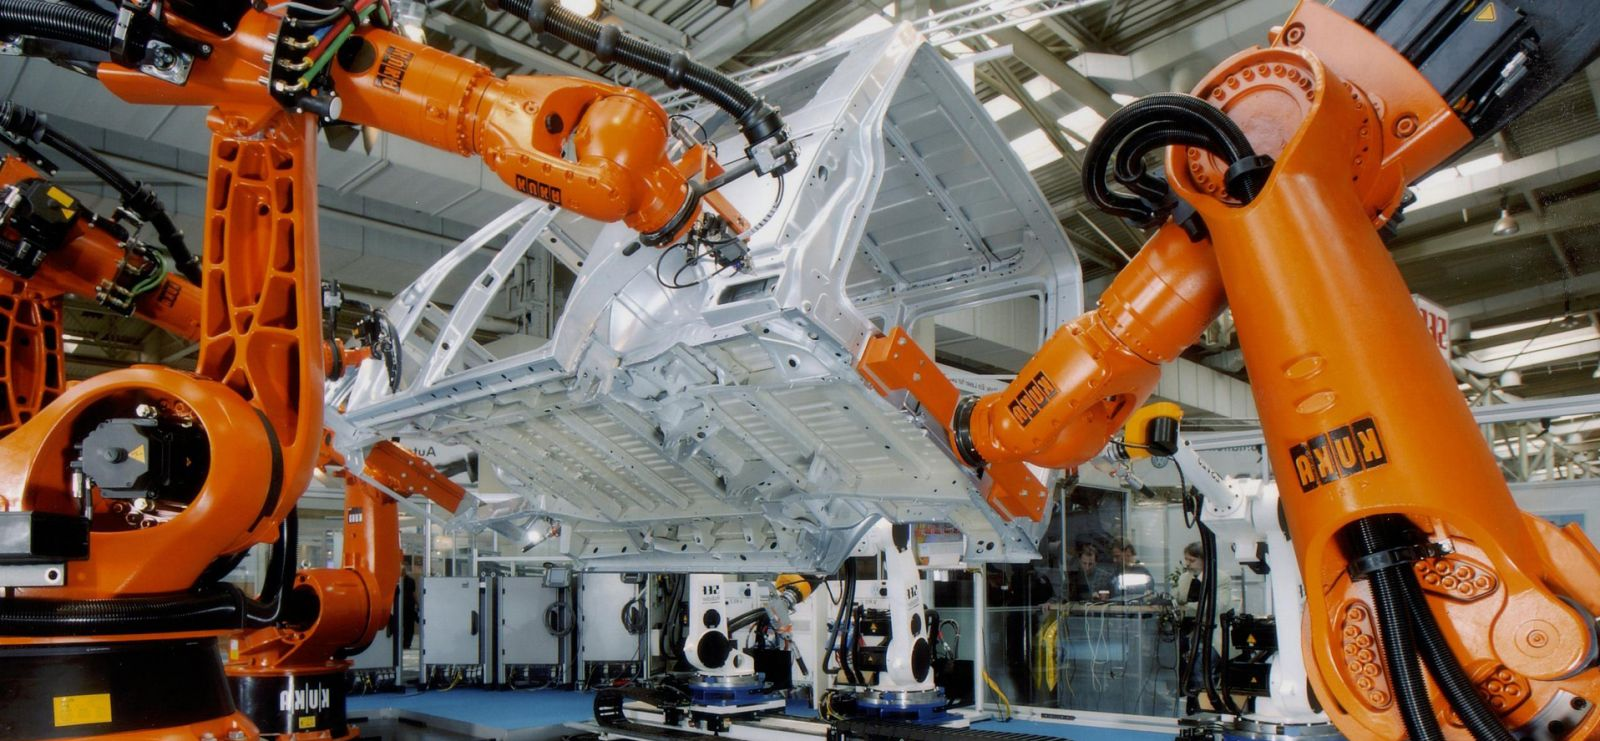
\includegraphics[height=.3\textheight]{kuka-heavy-assembly}
				\caption{Robots holding car}
			\end{minipage}
		\end{figure}
	\end{itemize}
\end{frame}


\subsection{Motivation}
\begin{frame}{Motivation}
	\begin{itemize}
		\item Teaching new assembly skills by demonstration can reduce the cost of re-purposing a robot for new tasks
		\item Cooperative assembly of complex objects can improve overall productivity
		\begin{itemize}
			\item Robot assembles components that it can quickly grasp and that need high assembly precision
			\item Human assembles the parts that the robot cannot grasp or the tasks that the robot takes more time than a human operator
		\end{itemize}
		\begin{figure}[!ht]
			\centering
			\begin{minipage}{.40\textwidth}
				\centering
				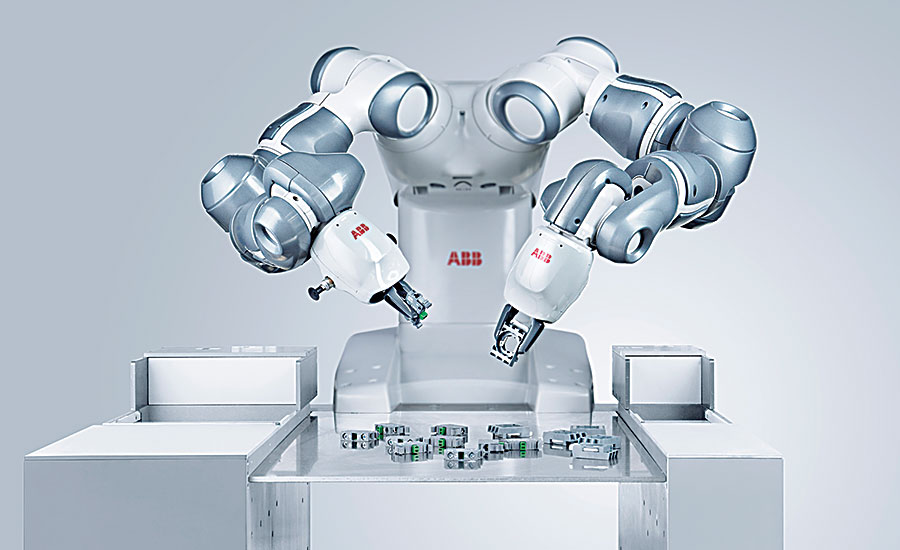
\includegraphics[height=.28\textheight]{yumi}
				\caption{ABB Yumi cooperative robot}
			\end{minipage}%
			\begin{minipage}{0.55\textwidth}
				\centering
				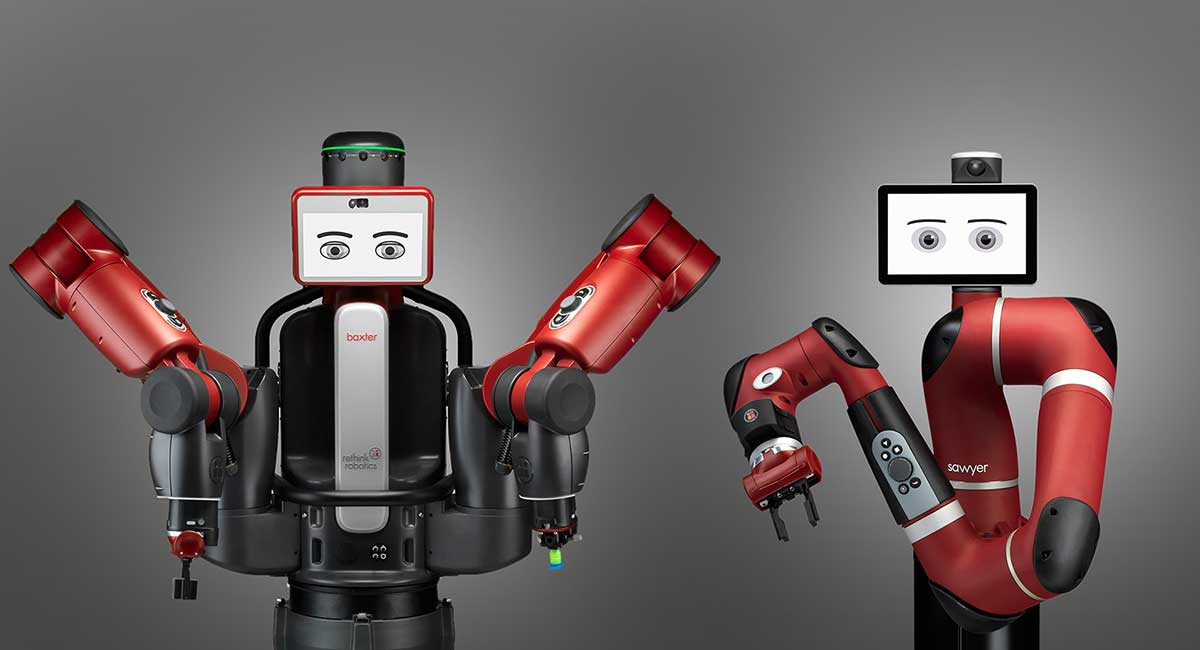
\includegraphics[height=.28\textheight]{rethink-robotics-baxter-sawyer}
				\caption{Rethink Robotics cooperative robots}
			\end{minipage}
		\end{figure}
	\end{itemize}
\end{frame}


\subsection{Research areas}
\begin{frame}{Research areas}
	\begin{itemize}
		\item Machine Learning
		\begin{itemize}
			\item Learning new semantic assembly skills by demonstration
		\end{itemize}
		\item Computer Vision, 3D perception and Human Machine Interface
		\begin{itemize}
			\item Recognition and tracking of assembly objects
			\item Detection of operator movements for semantic assembly analysis and user interface
			\item Human-robot cooperation
		\end{itemize}
		\item Augmented Reality
		\begin{itemize}
			\item Projection of information into the workspace to help the human operator
			\begin{itemize}
				\item Informing the operator which object it should pick and where it should assemble it
			\end{itemize}
		\end{itemize}
		\item Natural Language Processing
		\begin{itemize}
			\item Extraction of assembly information from instruction manuals
			\item Recognition of voice commands from the human operator
		\end{itemize}
	\end{itemize}
\end{frame}

\section{\scshape State of art}\label{sec:state-of-art}

\subsection{Related work}
\begin{frame}{Related work}
	\begin{itemize}
		\item Machine Learning
		\begin{itemize}
			\item Support Vector Machines
			\item Neural networks
			\item Hidden Markov Models
			\item Gaussian Mixture of Models
		\end{itemize}
		\item Computer Vision, 3D perception and Human Machine Interface
		\begin{itemize}
			\item Visual, geometric feature association
			\item Template, shape matching
			\item Color, intensity, texture segmentation
			\item Human-robot cooperation
		\end{itemize}
		\item Augmented Reality
		\begin{itemize}
			\item Projection mapping with DLP and laser projectors
		\end{itemize}
		\item Natural Language Processing
		\begin{itemize}
			\item N-gram models
		\end{itemize}
	\end{itemize}
\end{frame}

\subsection{Related work (hardware)}
\begin{frame}{Related work (hardware)}
	\begin{itemize}
		\item Robot manipulators
		\begin{itemize}
			\item Robotic arms
			\item Motion planners
			\item Robotic grippers
			\item Force control assembly
			\item Automatic tool change
			\item Environment fixtures
		\end{itemize}
		\item Perception sensors
		\begin{itemize}
			\item Image
			\item Stereo vision
			\item Camera-laser
			\item Structured light methods
			\item Time of Flight methods
		\end{itemize}
	\end{itemize}
\end{frame}

\subsection{Related work (software)}
\begin{frame}{Related work (software)}
	\begin{itemize}
		\item Frameworks
		\begin{itemize}
			\item Robot Operating System (ROS)
			\item Rapyuta
			\item OpenEASE
			\item CTAM
			\item RoboBrain
			\item KnowRob
		\end{itemize}
		\item Libraries
		\begin{itemize}
			\item Point Cloud Library (PCL)
			\item Open Computer Vision (OpenCV)
			\item Gazebo simulator
		\end{itemize}
	\end{itemize}
\end{frame}

\subsection{Main related research publications}
\begin{frame}{Main related research publications}
	\begin{itemize}
		\item Assembly operations
		\begin{itemize}
			\begingroup
			\scriptsize
			\item U. Thomas and F. M. Wahl, "A system for automatic planning, evaluation and execution of assembly sequences for industrial robots," Intelligent Robots and Systems, 2001. Proceedings. 2001 IEEE/RSJ International Conference on, Maui, HI, 2001, pp. 1458-1464 vol.3. \textbf{(seminal paper)}
			\item U. Thomas, F. M. Wahl, J. Maass and J. Hesselbach, "Towards a new concept of robot programming in high speed assembly applications," 2005 IEEE/RSJ International Conference on Intelligent Robots and Systems, 2005, pp. 3827-3833.
			\item U. Thomas, B. Finkemeyer, T. Kroger and F. M. Wahl, "Error-tolerant execution of complex robot tasks based on skill primitives," Robotics and Automation, 2003. Proceedings. ICRA '03. IEEE International Conference on, 2003, pp. 3069-3075 vol.3.
			\item U. Thomas, M. Barrenscheen and F. M. Wahl, "Efficient assembly sequence planning using stereographical projections of C-space obstacles," Assembly and Task Planning, 2003. Proceedings of the IEEE International Symposium on, 2003, pp. 96-102.
			\item D. Surdilovic, G. Schreck and U. Schmidt, "Development of Collaborative Robots (COBOTS) for Flexible Human-Integrated Assembly Automation," Robotics (ISR), 2010 41st International Symposium on and 2010 6th German Conference on Robotics (ROBOTIK), Munich, Germany, 2010, pp. 1-8.
			\endgroup
		\end{itemize}
	\end{itemize}
\end{frame}

%\subsection{Main related research publications}
\begin{frame}{}
	\begin{itemize}
		\item Robot arm control and path planning
		\begin{itemize}
			\begingroup
			\scriptsize
			\item C. Liu and M. Tomizuka, "Modeling and controller design of cooperative robots in workspace sharing human-robot assembly teams," 2014 IEEE/RSJ International Conference on Intelligent Robots and Systems, Chicago, IL, 2014, pp. 1386-1391.
			\item J. S. You, D. H. Kim, S. J. Lim, S. P. Kang, J. Y. Lee and C. S. Han, "Development of manipulation planning algorithm for a dual-arm robot assembly task," 2012 IEEE International Conference on Automation Science and Engineering (CASE), Seoul, 2012, pp. 1061-1066.
			\item U. Thomas and F. M. Wahl, "A system for automatic planning, evaluation and execution of assembly sequences for industrial robots," Intelligent Robots and Systems, 2001. Proceedings. 2001 IEEE/RSJ International Conference on, Maui, HI, 2001, pp. 1458-1464 vol.3.
			\endgroup
		\end{itemize}
		
		\item Human Machine Interface
		\begin{itemize}
			\begingroup
			\scriptsize
			\item A. Roitberg, A. Perzylo, N. Somani, M. Giuliani, M. Rickert and A. Knoll, "Human activity recognition in the context of industrial human-robot interaction," Signal and Information Processing Association Annual Summit and Conference (APSIPA), 2014 Asia-Pacific, Siem Reap, 2014, pp. 1-10.
			\endgroup
		\end{itemize}
	\end{itemize}
\end{frame}

\subsection{Main conferences and journals}
\begin{frame}{Main conferences and journals}
	\begin{itemize}
		\item Conferences
		\begin{itemize}
			\item ICRA - IEEE International Conference on Robotics and Automation
			\item IROS - IEEE/RSJ International Conference on Intelligent Robots and Systems
			\item ICCV - IEEE International Conference on Computer Vision
		\end{itemize}
		\item Journals
		\begin{itemize}
			\item International Journal of Robotics Research (SJR - 4.184)
			\item IEEE Transactions on Industrial Informatics (SJR - 2.973)
			\item IEEE Transactions on Robotics (SJR - 2.884)
			\item IEEE Robotics and Automation Magazine (SJR - 1.832)
			\item Robotics and Computer-Integrated Manufacturing (SJR - 1.621)
			\item Robotics and Autonomous Systems (SJR - 1.377)
		\end{itemize}
	\end{itemize}

\end{frame}

\subsection{Related research projects}
\begin{frame}{Related research projects}
	\begin{itemize}
		\item Saphari
		\begin{itemize}
			\item Safe and Autonomous Physical Human-Aware Robot Interaction
		\end{itemize}
		\item Rosetta
		\begin{itemize}
			\item RObot control for Skilled ExecuTion of Tasks in natural interaction with humans; based on Autonomy, cumulative knowledge and learning
		\end{itemize}
		\item JAHIR
		\begin{itemize}
			\item Joint-Action for Humans and Industrial Robots
		\end{itemize}
		\item Charm
		\begin{itemize}
			\item Collaborative, Human-focused, Assistive Robotics for Manufacturing
		\end{itemize}
		\item RoboEarth
		\item KnowRob
	\end{itemize}
\end{frame}

\subsection{Related research groups}
\begin{frame}{Related research groups}
	\begin{itemize}
		\item Aalborg Universitet
		\item DLR - Deutsches Zentrum für Luft- und Raumfahrt
		\item ETH Zurich
		\item fortiss
		\item Fraunhofer Institute for Manufacturing Engineering and Automation
		\item Lunds Universitet
		\item Technische Universität Chemnitz
		\item Technische Universität München
		\item TU/e
		\item Universität Bremen
	\end{itemize}
\end{frame}

%\subsection{Related research groups}
%\begin{frame}{Related research groups}
%	Text.
%\end{frame}

\section{\scshape Proposal}\label{sec:proposal}

\subsection{Research questions}
\begin{frame}{Research questions}
	\begin{itemize}
		\item How to reliably learn new assembly skills given that the tracking of the assembly objects will always have pose estimation errors and temporary occlusions by the operator?
		\item How to generalize a specific assembly skill and reuse it to perform similar tasks?
		\item How to efficiently coordinate complex assembly procedures between humans and robots in a shared work space?
	\end{itemize}
\end{frame}

\subsection{Objectives}
\begin{frame}{Objectives}
	\begin{itemize}
		\item Development of a cooperative assembly system capable of:
		\begin{itemize}
			\item Reliably learning by human demonstration
			\item Perform cooperative assembly tasks with human operators
			\item Help human operators perform their tasks faster by projecting assembly information into the workspace
			\begin{itemize}
				\item Showing which objects the human should pick up
				\item Where to place the objects with precision (no need for manual measurements)
				\item The order of assembly
			\end{itemize}
		\end{itemize}

	\end{itemize}
\end{frame}

\subsection{Applications}
\begin{frame}{Applications}
	\begin{itemize}
		\item Assembly of objects with increasing complexity, such as:
		\begin{itemize}
			\item Alternators
			\item Engines
			\item Gearboxes
		\end{itemize}
	\end{itemize}
	\begin{figure}[!ht]
		\centering
		\begin{minipage}{0.32\textwidth}
			\centering
			\includegraphics[height=.28\textheight]{gearbox}
			\caption{Gearbox parts}
		\end{minipage}%
		\begin{minipage}{.32\textwidth}
			\centering
			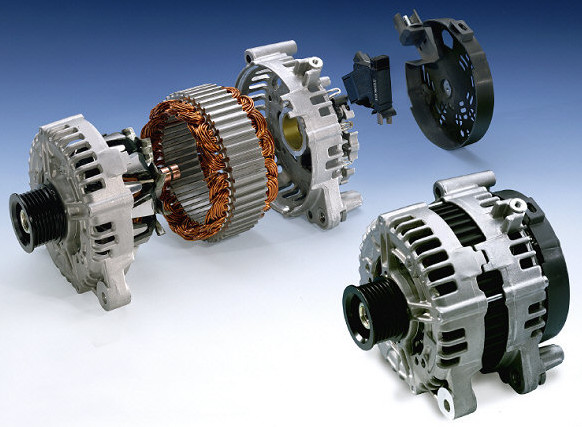
\includegraphics[height=.28\textheight]{alternator}
			\caption{Alternator parts}
		\end{minipage}%
		\begin{minipage}{0.32\textwidth}
			\centering
			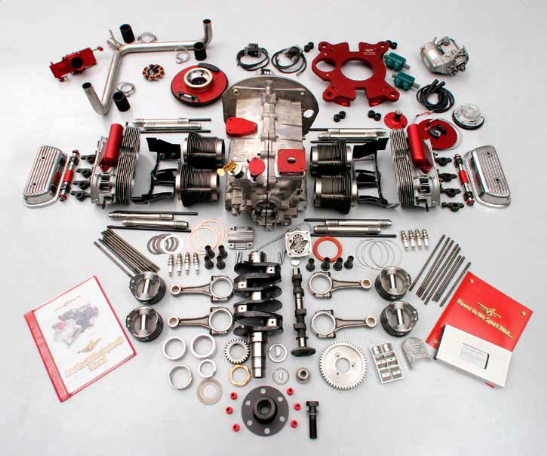
\includegraphics[height=.28\textheight]{engines}
			\caption{Engines parts}
		\end{minipage}
	\end{figure}
\end{frame}

\subsection{Methodology}
\begin{frame}{Methodology}
	\begin{itemize}
		\item Detailed description of the intended functionality and and final users of each software module
		\item Selection of the hardware and software platform in which the research will be performed
		\item Selection / creation of representative testing datasets for each of the main software modules
		\begin{itemize}
			\item 2d / 3D perception of geometry / objects and operator movements
			\item Learning new skills
			\item Human Machine Interface
		\end{itemize}
		\item Test and comparison of current state of the art methods for each software module
		\item Development of new / improved methods / algorithms when required
		\item Focus research on reliably learning new assembly skills
		\item Industrial testing of each software module with the final users
	\end{itemize}
\end{frame}

\section{\scshape Work plan}\label{sec:workplan}

\subsection{Milestones}
\begin{frame}{Milestones}
	\begin{itemize}
		\item Literature review (3 months)
		\item Setup of testing platforms (1 month)
		\item Creation of perception and learning datasets (2 month)
		\item Definition of system architecture (3 months)
		\item System implementation (26 months)
		\begin{itemize}
			\item Perception modules (4 months)
			\item Learning modules (7 months)
			\item Voice and gesture recognition modules (3 months)
			\item Augmented reality interface (4 months)
		\end{itemize}
		\item Validation of system in industrial conditions (6 months)
		\item Writing of articles and thesis (7 months)
	\end{itemize}
\end{frame}

\subsection{Gantt chart}
\begin{frame}{Gantt chart}
	\begin{figure}
		\centering
		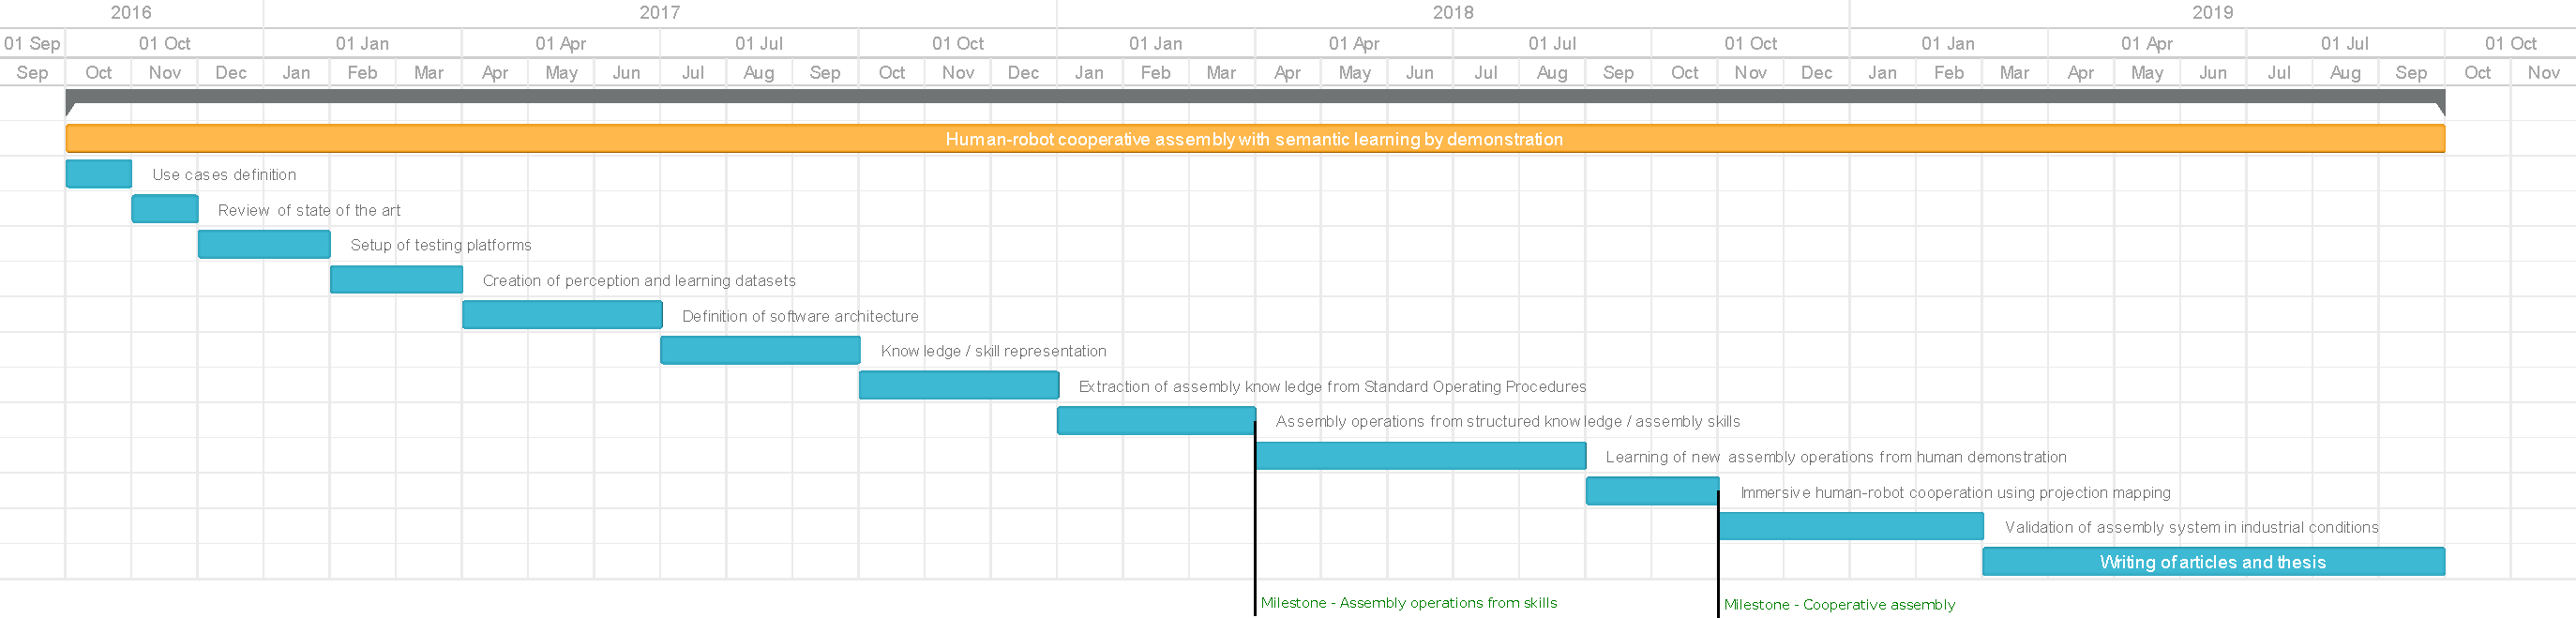
\includegraphics[width=\linewidth]{gantt-chart}
		\caption{Gantt chart}
	\end{figure}
\end{frame}

\section{\scshape Preliminary work}\label{sec:preliminary-work}

\begin{frame}{Preliminary work}
		\begin{figure}[!ht]
			\centering
			\begin{minipage}{.5\textwidth}
				\centering
				\includegraphics[height=.33\textheight]{projection-dlp-white}
			\end{minipage}%
			\begin{minipage}{0.5\textwidth}
				\centering
				\includegraphics[height=.33\textheight]{projection-dlp}
			\end{minipage}
			\caption{Projection mapping system for DLP projectors}
		\end{figure}%
		\begin{figure}[!ht]
			\centering
			\begin{minipage}{.5\textwidth}
				\centering
				\includegraphics[height=.33\textheight]{projection-object}
			\end{minipage}%
			\begin{minipage}{0.5\textwidth}
				\centering
				\includegraphics[height=.33\textheight]{projection-side}
			\end{minipage}
			\caption{Projection mapping system for laser projectors}
		\end{figure}
\end{frame}

%\section*{\scshape References}\label{sec:references}
%
%\subsection{References}
%\begin{frame}{References}
%	\begin{itemize}
%		\item [1]
%	\end{itemize}
%\end{frame}

\section*{}\label{sec:questions}

\begin{frame}{}
	\begin{center}
		\Huge
		Thank you!\\
		Questions?
	\end{center}
\end{frame}



\end{document}
